\begin{figure}
    \centering
    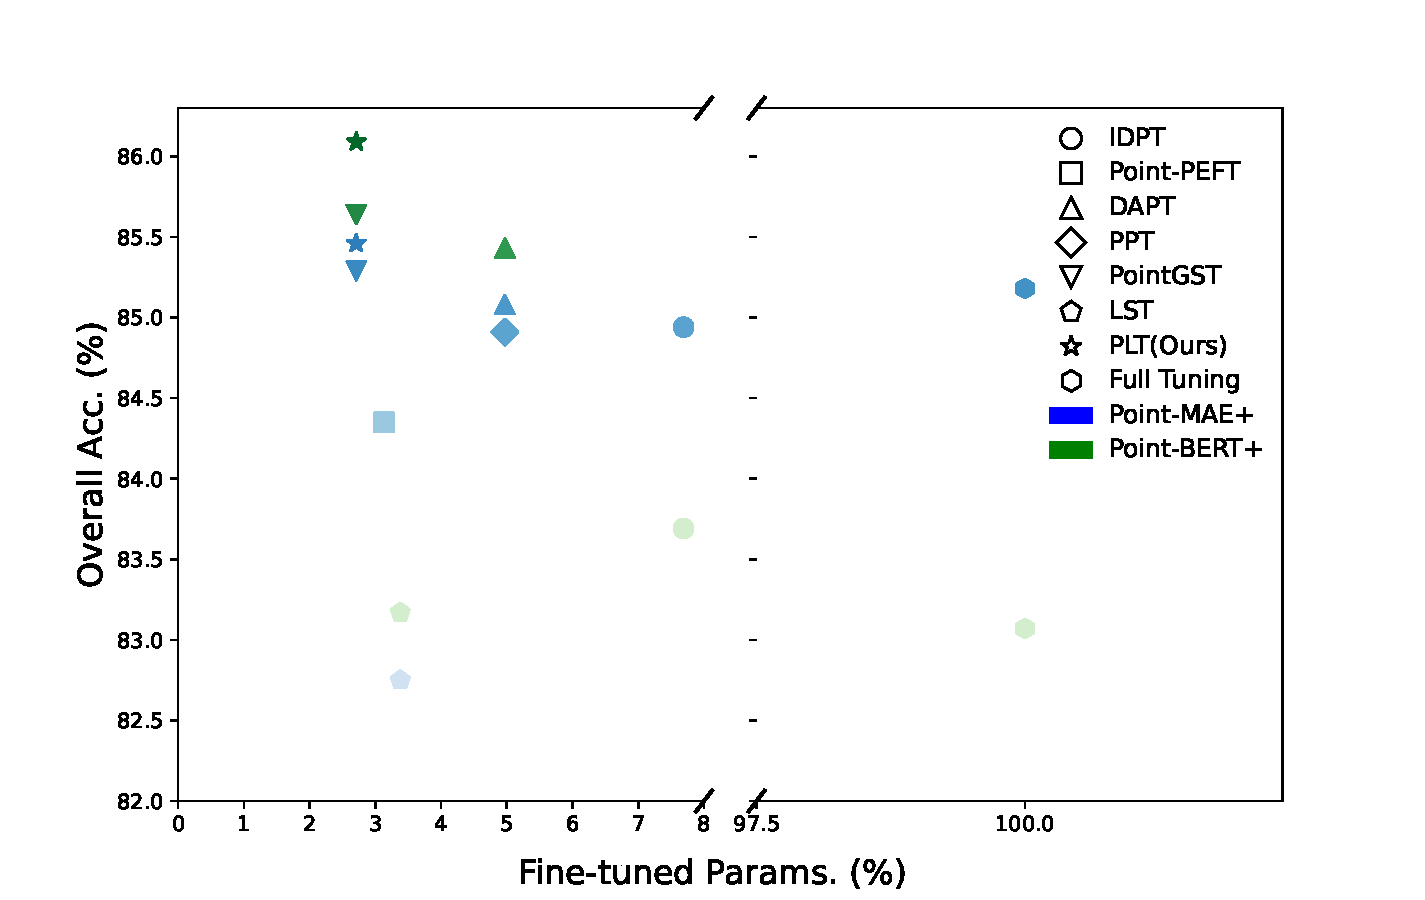
\includegraphics[width=\linewidth]{fig/sota.pdf}
    \caption{Comparison of various methods on the most challenging variant of ScanObjectNN~\cite{uy2019revisiting}. Different shapes indicate different methods, with blue and green representing results under the PointMAE~\cite{pang2022masked} and PointBERT~\cite{yu2022point} baselines, respectively. Darker colors correspond to higher accuracy, where accuracy values are normalized to the range [0,1] using max-min scaling~\cite{panda2014smoothing}.
}
    \label{fig:sota}
\end{figure}